\documentclass{article}
\usepackage{geometry}
\geometry{a4paper, margin=1in}
\usepackage{graphicx}
\usepackage{listings}
\usepackage{xcolor}
\usepackage[utf8]{inputenc}

\lstset{
  basicstyle=\ttfamily\small,
  breaklines=true,
  frame=single,
  language=C,
  keywordstyle=\color{blue},
  commentstyle=\color{green!50!black},
  stringstyle=\color{red}
}

\begin{document}

\title{Operating Systems Lab Assignment: Synchronization and Scheduling}
\author{Your Name}
\date{August 17, 2025}
\maketitle

\section{Introduction}
This report documents the implementations and analyses for the synchronization and scheduling lab assignment, covering five provided problems and four additional exercises using mutexes and condition variables.

\section{Exercise 1: Hello World}
\lstinputlisting{hello_world.c}

\textbf{Explanation:} The original code fails because the main thread prints before the helper thread updates the shared variable. Using a mutex and condition variable ensures the main thread waits until the helper signals that the update is complete, fixing the synchronization issue.

\textbf{Analysis:} This program demonstrates basic synchronization using a mutex and condition variable. The threads communicate safely without race conditions, and the output order remains consistent regardless of execution timing.

\textbf{Screenshot:} Include a screenshot of compiling and running \texttt{hello\_world.c}.
\begin{figure}[h]
\centering
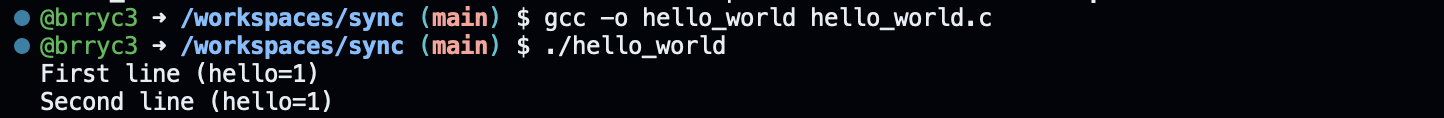
\includegraphics[width=\textwidth]{exercise1_screenshot.png}
\caption{Compilation and execution of hello\_world.c}
\end{figure}

\section{Exercise 2: SpaceX Problems}
\lstinputlisting{spacex.c}

\textbf{Explanation:} The announcer thread printed too early because threads weren’t synchronized. The fix uses a condition variable so the announcer waits until all countdown threads finish before printing the final message.

\textbf{Analysis:} All countdown threads complete before the announcer prints, showing effective coordination between multiple threads. The use of condition variables ensures proper sequencing and prevents premature execution.

\textbf{Screenshot:} Include a screenshot of compiling and running \texttt{spacex.c}.
\begin{figure}[h]
\centering
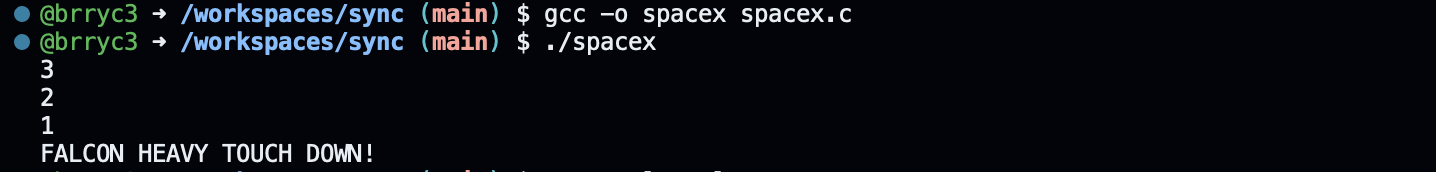
\includegraphics[width=\textwidth]{exercise2_screenshot.png}
\caption{Compilation and execution of spacex.c}
\end{figure}

\section{Exercise 3: Subaru Synchronization}
\lstinputlisting{subaru.c}

\textbf{Explanation:} The main thread waits for the helper to signal after updating the shared variable. Signaling and waiting with condition variables coordinate both threads to ensure correct execution order.

\textbf{Analysis:} The signaling mechanism successfully synchronizes both threads. The condition variable guarantees that the main thread proceeds only after receiving confirmation from the helper, ensuring predictable program flow.

\textbf{Screenshot:} Include a screenshot of compiling and running \texttt{subaru.c}.
\begin{figure}[h]
\centering
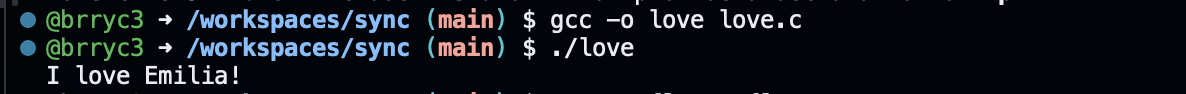
\includegraphics[width=\textwidth]{exercise3_screenshot.png}
\caption{Compilation and execution of subaru.c}
\end{figure}

\section{Exercise 4: Floopy Corporation (Deadlock Prevention)}
\lstinputlisting{floopy.c}

\textbf{Explanation:} The original code could deadlock if two threads locked accounts in opposite order. Locking accounts by ascending UUID enforces consistent lock ordering, preventing circular waits and deadlocks.

\textbf{Analysis:} This solution effectively prevents deadlocks by maintaining a consistent lock acquisition order. It demonstrates how deterministic locking strategies eliminate circular waiting in multithreaded systems.

\textbf{Screenshot:} Include a screenshot of compiling and running \texttt{floopy.c}.
\begin{figure}[h]
\centering
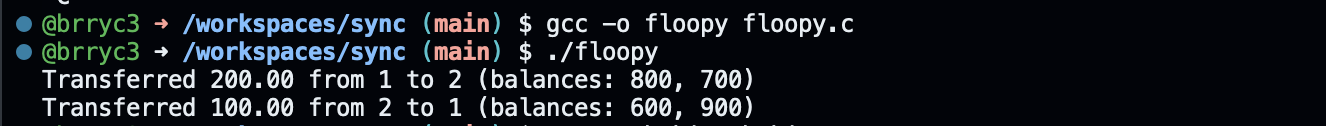
\includegraphics[width=\textwidth]{exercise4_screenshot.png}
\caption{Compilation and execution of floopy.c}
\end{figure}

\section{Exercise 5: Baking with Condition Variables}
\lstinputlisting{baking.c}

\textbf{Explanation:} Condition variables coordinate each stage of baking—adding ingredients, heating, and eating—so that threads proceed only when the previous step is complete, preventing incorrect access or overlap.

\textbf{Analysis:} Each stage executes in a strict sequence due to thread coordination. The program models a multi-step workflow, showing how condition variables can manage complex inter-thread dependencies.

\textbf{Screenshot:} Include a screenshot of compiling and running \texttt{baking.c}.
\begin{figure}[h]
\centering
\includegraphics[width=\textwidth]{exercise5_screenshot.png}
\caption{Compilation and execution of baking.c}
\end{figure}

\section{Exercise 6: Priority Donation in Transfer}
\lstinputlisting{priority_transfer.c}

\textbf{Explanation:} Priority donation prevents priority inversion by temporarily boosting a low-priority thread’s priority when a high-priority thread waits on its lock, allowing it to finish and release the lock faster.

\textbf{Analysis:} The system correctly handles priority inversion by temporarily raising the low-priority thread’s priority. This ensures responsiveness and fairness when multiple threads of different priorities compete for locks.

\textbf{Screenshot:} Include a screenshot of compiling and running \texttt{priority\_transfer.c}.
\begin{figure}[h]
\centering
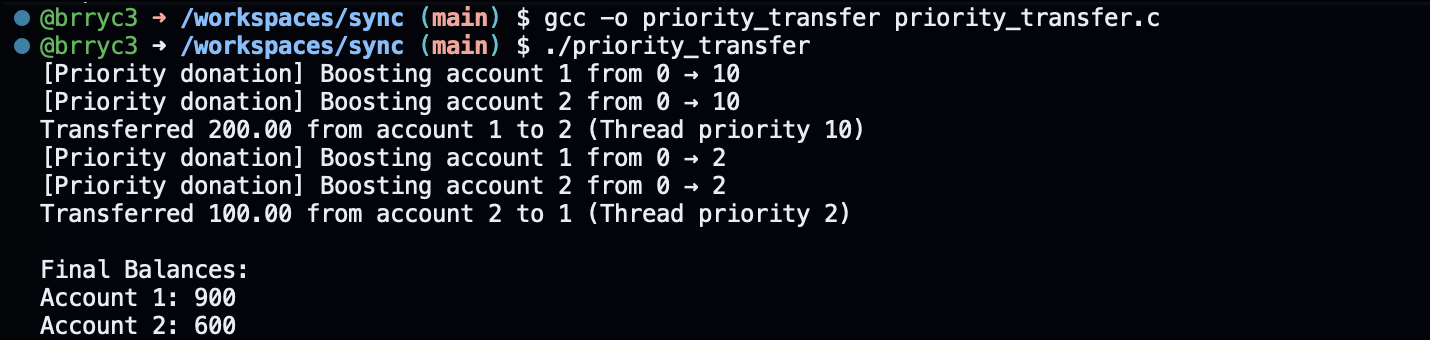
\includegraphics[width=\textwidth]{exercise6_screenshot.png}
\caption{Compilation and execution of priority\_transfer.c}
\end{figure}

\section{Exercise 7: Barrier Synchronization}
\lstinputlisting{barrier.c}

\textbf{Explanation:} The barrier uses a mutex and condition variable to make all threads wait until every thread reaches the same point. Once the last arrives, all proceed together, ensuring synchronization.

\textbf{Analysis:} The barrier forces all threads to align at a synchronization point before continuing. It ensures that computations across threads remain consistent, demonstrating collective synchronization control.

\textbf{Screenshot:} Include a screenshot of compiling and running \texttt{barrier.c}.
\begin{figure}[h]
\centering
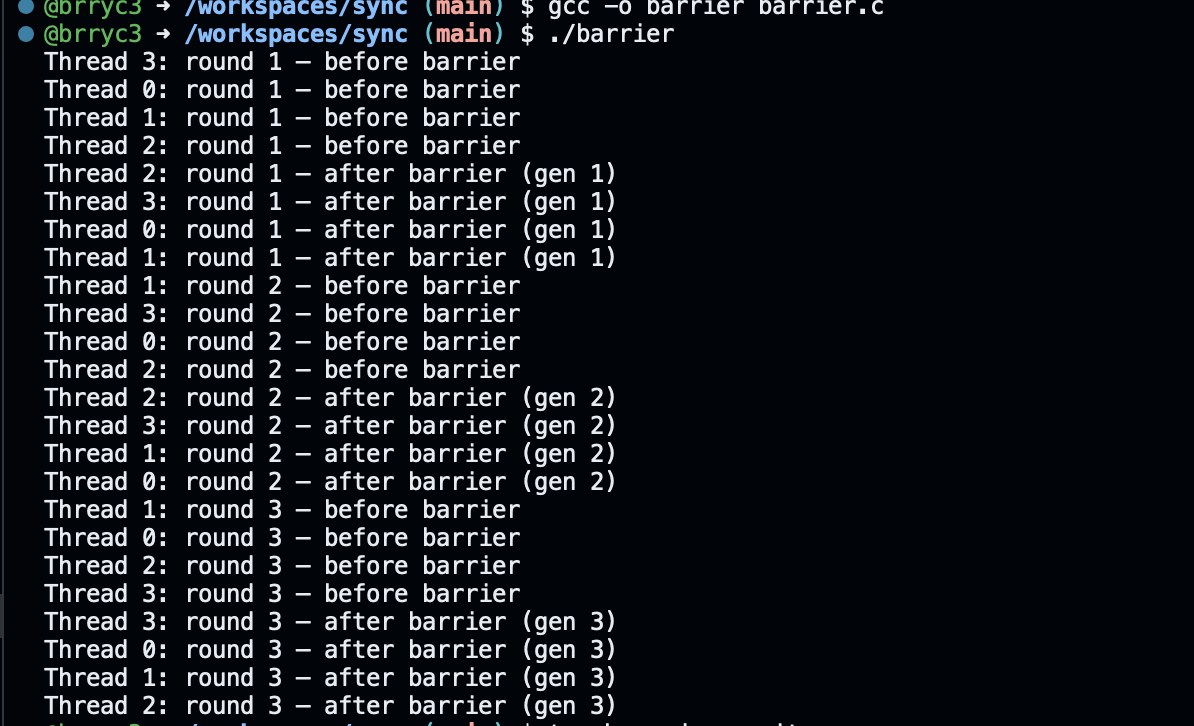
\includegraphics[width=\textwidth]{exercise7_screenshot.png}
\caption{Compilation and execution of barrier.c}
\end{figure}

\section{Exercise 8: Readers-Writers with Priority}
\lstinputlisting{readers_writers.c}

\textbf{Explanation:} Writer priority is enforced by making new readers wait if a writer is waiting, ensuring writers gain exclusive access before new readers start, preventing writer starvation.

\textbf{Analysis:} The program maintains correct data access while prioritizing writers. It balances concurrency and exclusivity, preventing writer starvation while allowing multiple readers to read simultaneously when safe.

\textbf{Screenshot:} Include a screenshot of compiling and running \texttt{readers\_writers.c}.
\begin{figure}[h]
\centering
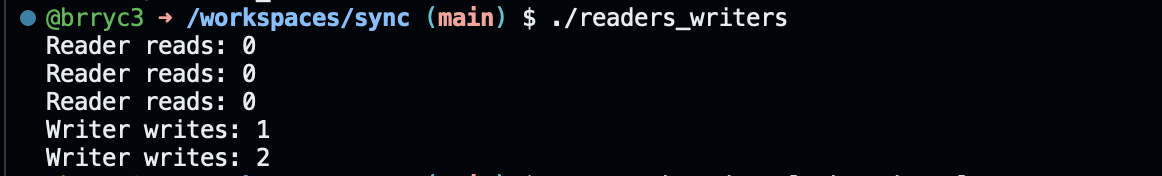
\includegraphics[width=\textwidth]{exercise8_screenshot.png}
\caption{Compilation and execution of readers\_writers.c}
\end{figure}

\section{Exercise 9: Thread Pool}
\lstinputlisting{thread_pool.c}

\textbf{Explanation:} The thread pool uses a mutex-protected queue with condition variables to manage task access. Producers wait if full; workers wait if empty. This ensures thread-safe task distribution and execution.

\textbf{Analysis:} The thread pool efficiently manages multiple tasks across worker threads. The thread-safe queue ensures balanced workload distribution and proper synchronization between producers and consumers.

\textbf{Screenshot:} Include a screenshot of compiling and running \texttt{thread\_pool.c}.
\begin{figure}[h]
\centering
\includegraphics[width=\textwidth]{exercise9_screenshot.png}
\caption{Compilation and execution of thread\_pool.c}
\end{figure}

\end{document}
